abbreviations\chapter{Some useful tips on your thesis}

Below, I describe several technical moments on formatting your thesis. 
\section{Fontsize}

Keep the fontsize in the dissertation settings. You can use a font size of 12 pt for tables, but smaller sizes are not permitted. 

The rules do not standardize the font on the figures, but all inscriptions on the figures must be clearly readable.

\section{Equations}

\textbf{All} equations should be numbered, even if you do not plan to refer to them. 

The \textbf{\textcolor{red}{wrong}} version:
\[2 + 2 = 4\]

The \textbf{\textcolor{green}{correct}} version:
\begin{equation}
	2 + 2 = 4
\end{equation}

\section{Figures}

\textbf{All} figures should be \textbf{referred in the text body}. The reference should appear \textbf{before} the figure. The figure must not interrupt the paragraph. 

\textcolor{red}{\textbf{Wrong version.}} The Skolkovo Institute of Science and Technology (Skoltech) is a private graduate research university in Moscow that has rapidly emerged as a key player in Russia's drive for scientific and technological advancement. 
\begin{figure}[!h]
	\centering
	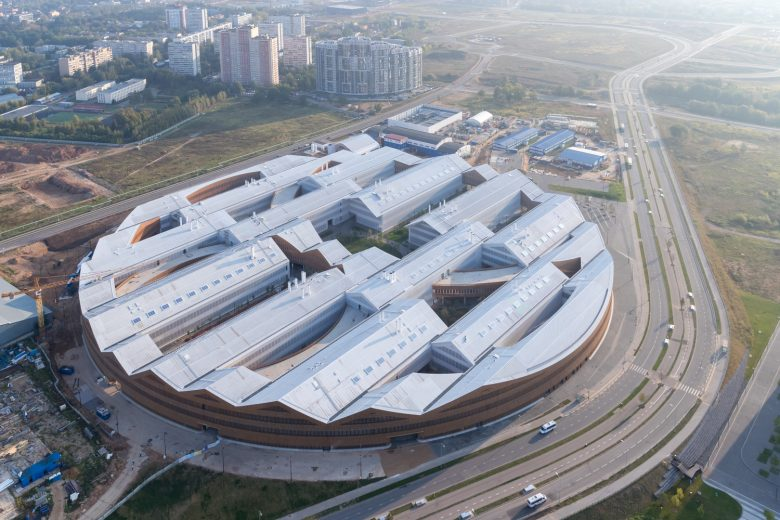
\includegraphics[width=0.5\textwidth]{skoltech.jpg}
	\caption{Skoltech. The figure appears before the corresponding reference. This figure interrupts the paragraph.}
	\label{fig:example}
\end{figure}
Established in 2011 in collaboration with the Massachusetts Institute of Technology (MIT), Skoltech was conceived as the cornerstone of the Skolkovo Innovation Center, a high-tech business area aimed at fostering a vibrant ecosystem of entrepreneurship and innovation.

\textcolor{green}{\textbf{Correct version.}}
Instruction at Skoltech, depicted on Figure~\ref{fig:example}, is conducted entirely in English, attracting an international body of students and faculty. The university offers Master of Science (MSc) and Doctor of Philosophy (PhD) degrees across a range of fields, including data science, artificial intelligence, mathematics, physics, materials science, life sciences, and engineering systems. A strong emphasis is placed on integrating research, education, and innovation. 

\begin{figure}[!h]
	\centering
	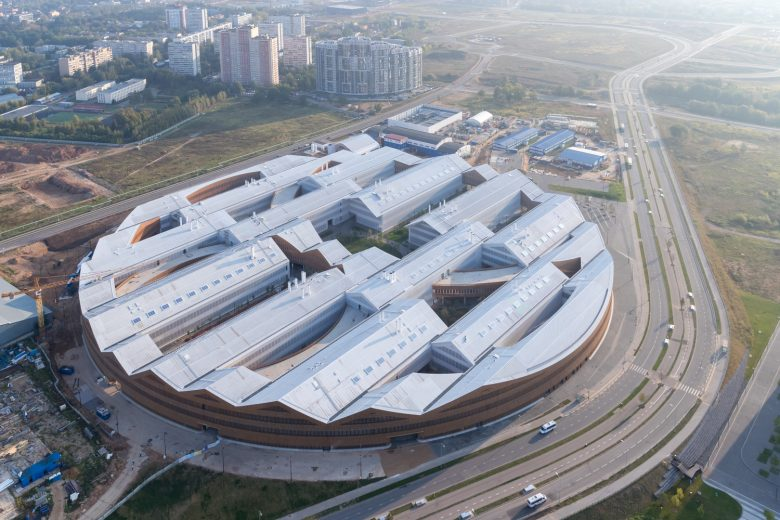
\includegraphics[width=0.5\textwidth]{skoltech.jpg}
	\caption{Skoltech. The figure appears after the corresponding reference. This figure do not interrupt the paragraph.}
	\label{fig:example}
\end{figure}

\section{Tables}

If your table does not fit on the page in portrait format, you can use \textbf{landscape} format. Do not try to reduce table size by reducing font size or by using something like adjustbox instead. 

\section{References}
\textit{Here is the text for references generation~\cite{lorden1971procedures, zhang2024self, ширяев1965некоторые}}.

Firstly, sometimes you can see [0] instead of all references. Just rerun the compilation. You probably need to do it several times. It is also useful to delete the dissertation.aux file and rerun the compilation "from scratch". 

The next one is that the automatic generation of a list of an author's publication work is poor; thus, it is probably better to create the list manually. 

Then, you should refer to Russian-language literature~\cite{ширяев1965некоторые} separately from non-Russian language literature~\cite{lorden1971procedures, zhang2024self} (first non-Russian, then all Russian). This tool was not implemented in the original template, so I have implemented it crudely (check TODOs in biblio/biblatex). If you know how to improve it, please feel free to share your suggestions.  

Another issues is a weird format of references (see \href{https://github.com/aleksey-uvarov/Russian-English-PhD-LateX/blob/master/Readme/Bibliography.md}{comments}). For publications with fewer than three authors~\cite{lorden1971procedures}, you will see their names at the beginning of the reference. If there are more than three authors~\cite{zhang2024self}, you will see the title of the paper before the names of the authors. 
Although it is somewhat a GOST format, I was recommended to fix this behaviour. Unfortunately, I was not able to find how to do it. So, feel free to share your solutions. 

Last but not least is the automatic reference counting for the Introduction section. Due to the poor realization of the separation of Russian-language literature, it is broken. I did it just manually. 

\section{List of abbreviations}
Check \href{https://github.com/AndreyAkinshin/Russian-Phd-LaTeX-Dissertation-Template/blob/33420d8817f8cb0e3c1d2610a9c996212e2f80bb/Dissertation/part1.tex#L540}{\textbf{this one}} to familiarize yourself with various methods for generating a list of acronyms. 
 
\section{Final words}
You can find more useful tips and scenarios in the original \href{https://github.com/aleksey-uvarov/Russian-English-PhD-LateX/}{\textbf{repository}}. Feel free to improve this version; please do not hesitate to raise any issues or ask questions. 

